\textbf{COLUNI 2026 -- Questão 28}\par\medskip Em uma única árvore da Floresta Atlântica, como na foto abaixo, observamos uma comunidade integrada de diversos seres vivos. Variedades de pássaros, pequenos répteis, pequenos mamíferos e de insetos, como formigas, pulgões e cupins, morando e se alimentando entre as folhas e em galhos, ramos e no tronco. Orquídeas, bromélias e ervas-de-passarinho vivendo sobre os galhos e o tronco. Também sobre o tronco, líquens e musgos e, associados às raízes, os fungos. É uma diversidade enorme de vida!

\begin{figure}[htbp]
\centering
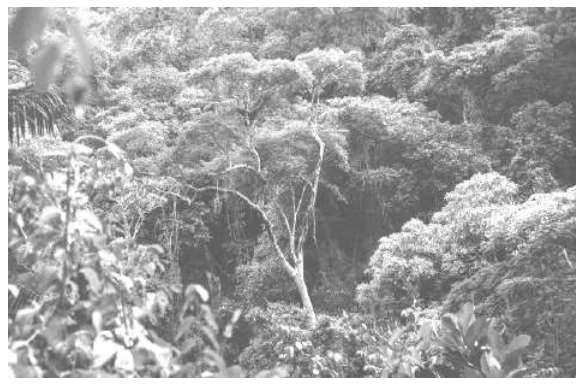
\includegraphics[width=0.72\linewidth]{static/simulados/coluni/figuras/2026/questao-28/figura-1.png}
\end{figure}

Disponível em: https://brasilescola.uol.com.br/biologia/mata-atlantica.html. Acesso em: 19 ago. 2025.

As espécies citadas apresentam muitas relações ecológicas entre elas e algumas dessas relações estão listadas abaixo:
\begin{itemize}
\item As formigas levam os pulgões aos seus formigueiros e os dominam para se alimentarem de suas excreções ricas em açúcar;
\item As ervas-de-passarinho, nos galhos, utilizam da seiva bruta da árvore;
\item As orquídeas e bromélias utilizam os troncos da árvore como suporte e moradia;
\item Alguns fungos nas raízes, as micorrizas, auxiliam na absorção de nutrientes para a árvore;
\item Pequenos micos se alimentam de frutos da árvore;
\item Os líquens fazem fotossíntese sobre o tronco da árvore;
\item Os cupins se alimentam da madeira rica em celulose.
\end{itemize}
O cupim consegue aproveitar a celulose como fonte de nutrientes, pois estabelece uma relação com microrganismos moradores de seu tubo digestivo. Esses microrganismos produzem uma enzima capaz de digerir a celulose e liberar nutrientes para o cupim.

Considerando as relações citadas acima, aquela que equivale CORRETAMENTE à relação ecológica entre o cupim e os microrganismos que digerem a celulose para ele é a relação entre:\begin{enumerate}
\item as ervas-de-passarinho e a árvore onde a erva vive em seus galhos.
\item as orquídeas e a árvore onde a orquídea vive sobre seu tronco.
\item os fungos e a árvore onde os fungos vivem em suas raízes.
\item os micos e a árvore de onde eles obtêm os frutos como alimento.\end{enumerate}